\documentclass[aspectratio=169]{beamer}
\beamertemplatenavigationsymbolsempty

\usepackage{parskip, setspace}
\setstretch{1.25}

\usepackage{biblatex}
\addbibresource{bib.bib}
% math formatting
\usepackage{amsmath, amsfonts, braket}
% \numberwithin{equation}{section}
% rich text
\usepackage{graphicx, caption}
\usepackage{hyperref}
\usepackage{xcolor}
\hypersetup{
    colorlinks=true,
    linkcolor=black,  
    urlcolor=blue,
    citecolor=blue,
    pdftitle={A Survey of Computational Physics},
    pdfpagemode=FullScreen
}

\usepackage[ruled,linesnumbered,lined,boxed,commentsnumbered]{algorithm2e}

\usetheme{Madrid}
\title[Quantum Computing]{Quantum Computing}
% \subtitle{}

\author[Chapman, Nathan]{Nathan Chapman}

\institute[CWU]
{
  Faculty of Physics\\
  Central Washington University
%   \and
%   \inst{2}%
%   Faculty of Chemistry\\
%   Very Famous University
}

\date[HPC 2024]{CS 530: High Performance Computing, Spring 2024}

\logo{
\includegraphics[height=0.5cm]{images/cwu_logo.png}}

\begin{document}

\frame{\titlepage}

\begin{frame}
    \frametitle{Why do we care?}
    \begin{columns}
        \begin{column}{0.5\textwidth}
            \begin{itemize}
                \item Because it's cool
                \item It turns out quantum computers can easily break classical cryptography
            \end{itemize}
        \end{column}
        \begin{column}{0.5\textwidth}
            
        \end{column}
    \end{columns}
\end{frame}

\begin{frame}
    \frametitle{Qubits - Heads or Tails?}

    \centering
    Does a coin show heads or tails?

\end{frame}

\begin{frame}
    \frametitle{Qubits - Single}
    \begin{columns}
        \begin{column}{0.5\textwidth}
            \begin{itemize}
                \item Classical - ``Bit''
                    \begin{itemize}
                        \item State is true or false
                        \item Always
                    \end{itemize}
                \item Quantum - ``Qubit''
                    \begin{itemize}
                        \item State is true or false or tralse or frue
                        \item State is a little bit of both
                        \item Until measured
                        \item At measurement, the state is true or false
                        % \item Example
                        % \begin{itemize}
                        %     \item Quantum Coin
                        %     \item $\ket{+} = \frac{1}{\sqrt{2}} \ket{0} + \frac{1}{\sqrt{2}} \ket{1}$
                        %     \item 50-50 probability
                        % \end{itemize}
                    \end{itemize}
                \item Example - A simple coin
                    \begin{itemize}
                        \item Classical - Deterministic via applied force, torque, height, etc.
                        \item Quantum - Probabilistic until measured
                    \end{itemize}
            \end{itemize}
        \end{column}
        \begin{column}{0.5\textwidth}
            \begin{figure}[h]
                \centering
                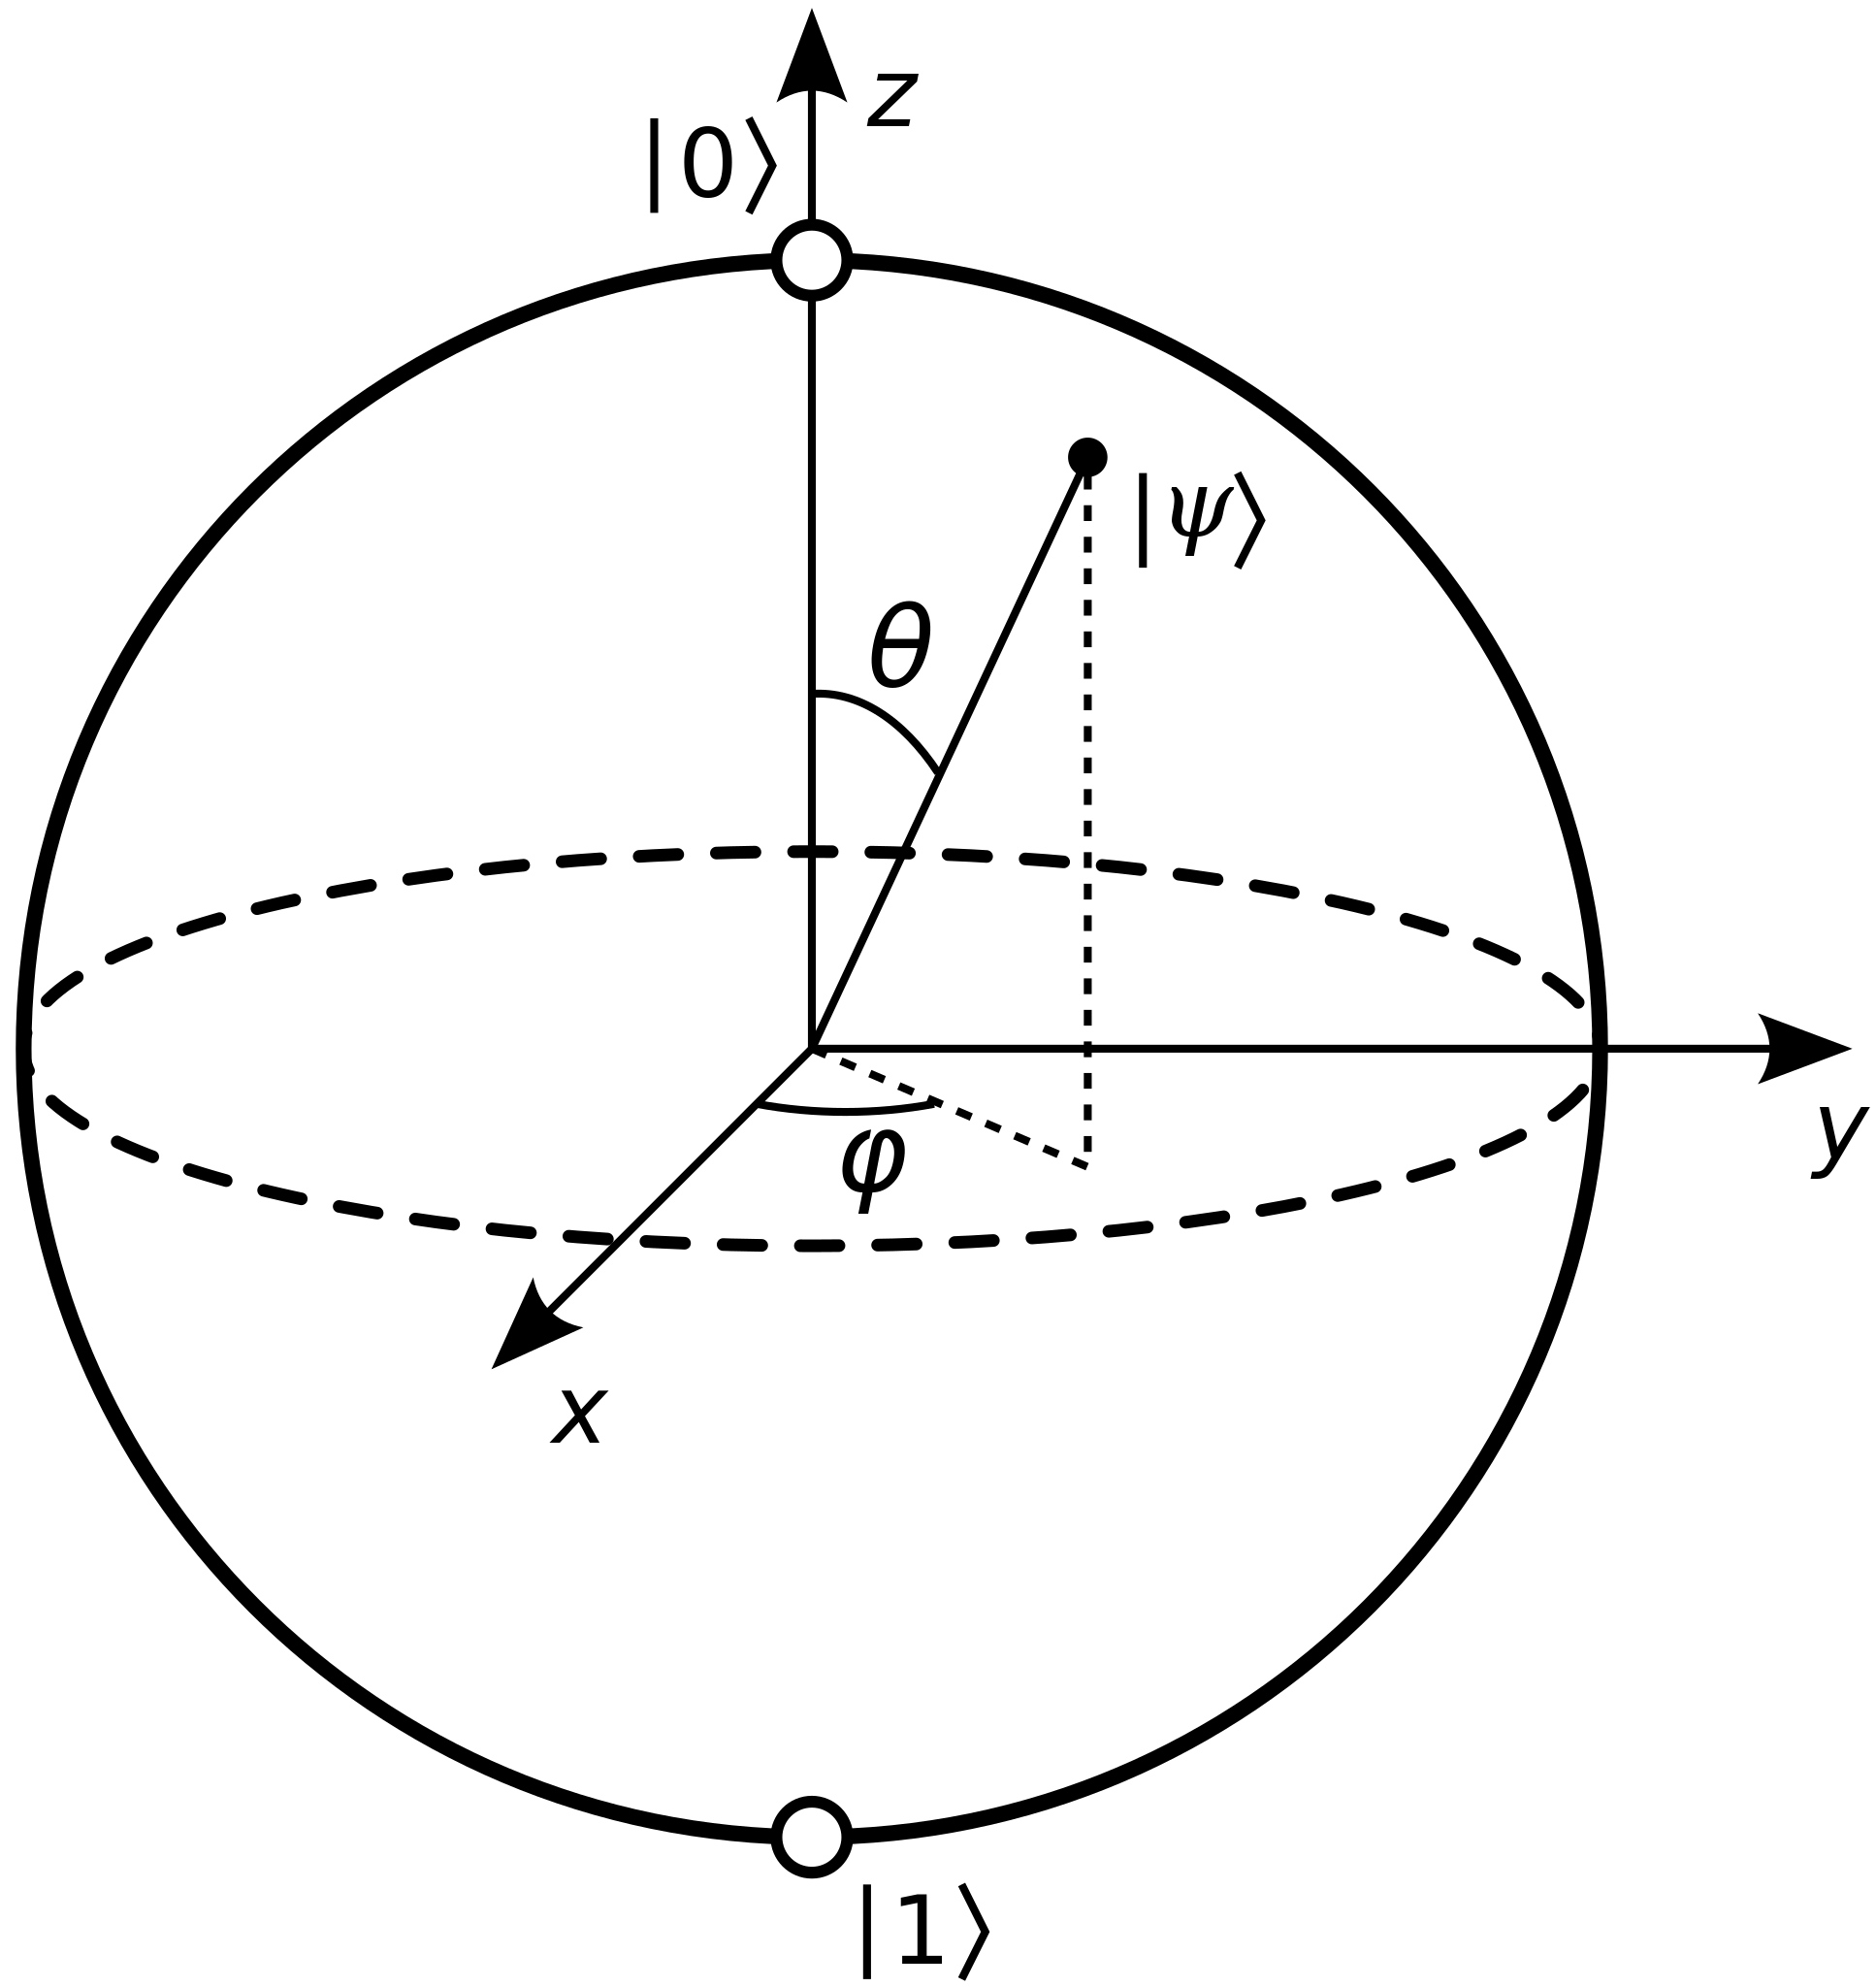
\includegraphics[height=0.7\textheight]{images/Bloch_sphere.png}
                \caption{The Bloch sphere reprensetation of a qubit \\ $\ket{\psi} = \cos \left( \frac{\theta}{2} \right) \ket{0} + e^{i \phi} \sin \left( \frac{\theta}{2} \right) \ket{1}$}
            \end{figure}
        \end{column}
    \end{columns}
\end{frame}

\begin{frame}
    \frametitle{Qubits - Multiple}
    \begin{columns}
        \begin{column}{0.5\textwidth}
            \begin{itemize}
                \item 2 qubits $\implies$ state is a mix between the 4 permutations $\{\ket{00}, \ket{01}, \ket{10}, \ket{11} \}$
                \item Each permutation has its own probability such that the total is 1
                \item Measure only qubit $\implies$ state renormalizes to only include remaining possible states
                \item Bell State: $50\% \ket{00}$ and $50\% \ket{11}$
            \end{itemize}
        \end{column}
        \begin{column}{0.5\textwidth}
            \centering Demo: 2 quantum coins with a volunteer
        \end{column}
    \end{columns}
\end{frame}

\begin{frame}
    \frametitle{Qubits - Quantum Registers}
    \begin{columns}
        \begin{column}{0.5\textwidth}
            \centering{\underline{Classical}}
            \begin{itemize}
                \item Register of size $N \equiv N$ flip-flops
                \item Stores 1 permutation of states
            \end{itemize}
        \end{column}
        \begin{column}{0.5\textwidth}
            \centering{\underline{Quantum}}
            \begin{itemize}
                \item Register of size $N$ $\equiv$ $N$ qubits
                \item Stores ALL $2^N$ permutations of states
            \end{itemize}
        \end{column}
    \end{columns}
    \begin{block}{}
        \centering The information density of a quantum computer can be massive
    \end{block}
\end{frame}

\begin{frame}
    \frametitle{Quantum Computation - Single Qubit Gates}
    \begin{columns}
        \begin{column}{0.5\textwidth}
            \centering{\underline{Classical}}
            \begin{itemize}
                \item Only one non-trivial gate
                \item NOT - $0 \to 1$
            \end{itemize}
        \end{column}
        \begin{column}{0.5\textwidth}
            \centering{\underline{Quantum}}
            \begin{itemize}
                \item Several non-trivial gates
                \item NOT (X) - swaps the probabilities
                \item Z - flips the sign of the probability on the $\ket{1}$ state
                \item Hadamard - ``mixes'' the pure states toward the other
                    \begin{itemize}
                        \item $\ket{0} \to 50\% \ket{0}$ and $50\% \ket{1}$
                        \item $\ket{1} \to 50\% \ket{0}$ and $-50\% \ket{1}$
                    \end{itemize}
            \end{itemize}
        \end{column}
    \end{columns}
\end{frame}

\begin{frame}
    \frametitle{Quantum Computation - Single Bit Gates}
    \begin{figure}[h]
        \centering
        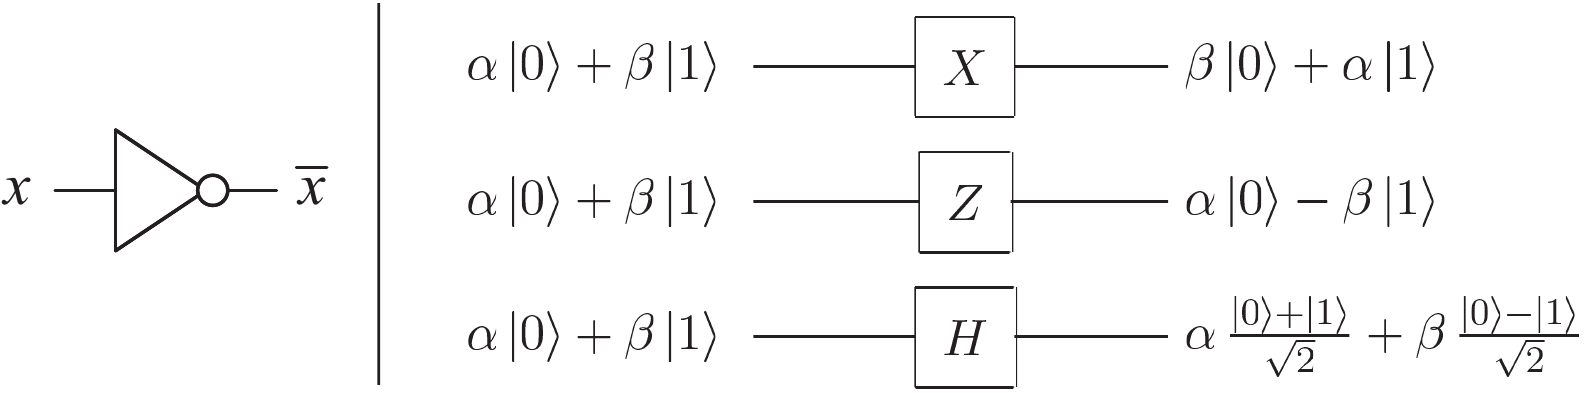
\includegraphics[width=0.9\textwidth]{images/single_circuits.png}
        \caption{A comparison between logic gates that can act on a single classical or quantum bit.}
    \end{figure}
\end{frame}

\begin{frame}
    \frametitle{Quantum Computation - Multi-Qubit Gates}
    \begin{columns}
        \begin{column}{0.5\textwidth}
            \centering{\underline{Classical}}
            \begin{itemize}
                \item AND, OR, XOR, NAND, NOR
                \item[]
                \item[]
                \item[] 
                \item XOR isn't invertible
                \item NAND makes up all gates
            \end{itemize}
        \end{column}
        \begin{column}{0.5\textwidth}
            \centering{\underline{Quantum}}
            \begin{itemize}
                \item Controlled not - CNOT
                \item Uses a \emph{control} bit and a \emph{target}
                \item If control is 1, NOT target, otherwise do nothing
                \item CNOT is invertible
                \item CNOT and single-gates make up all multi-gates
            \end{itemize}
        \end{column}
    \end{columns}
    \begin{alertblock}{}
        \centering Quantum gates need to conserve information
    \end{alertblock}
\end{frame}

\begin{frame}
    \frametitle{Quantum Computation - Circuits}
    \begin{columns}
        \begin{column}{0.5\textwidth}
            
        \end{column}
        \begin{column}{0.5\textwidth}
            
        \end{column}
    \end{columns}
\end{frame}

\begin{frame}
    \frametitle{Quantum Algorithms - The Quantum Fourier Transform}
    \begin{columns}
        \begin{column}{0.5\textwidth}
            
        \end{column}
        \begin{column}{0.5\textwidth}
            
        \end{column}
    \end{columns}
\end{frame}

\begin{frame}
    \frametitle{Quantum Algorithms - Quantum Search}
    \begin{columns}
        \begin{column}{0.5\textwidth}
            
        \end{column}
        \begin{column}{0.5\textwidth}
            
        \end{column}
    \end{columns}
\end{frame}

\begin{frame}
    \frametitle{Quantum Cryptography}
    \begin{columns}
        \begin{column}{0.5\textwidth}
            
        \end{column}
        \begin{column}{0.5\textwidth}
            
        \end{column}
    \end{columns}
\end{frame}

\begin{frame}
    \frametitle{Demo - Qiskit}
    \begin{columns}
        \begin{column}{0.5\textwidth}
            
        \end{column}
        \begin{column}{0.5\textwidth}
            
        \end{column}
    \end{columns}
\end{frame}

\begin{frame}
    \frametitle{Honorable Mention - CUDA-Q}
    \begin{columns}
        \begin{column}{0.5\textwidth}
            
        \end{column}
        \begin{column}{0.5\textwidth}
            
        \end{column}
    \end{columns}
\end{frame}

\begin{frame}
    \frametitle{Conclusion}

    

\end{frame}

\end{document}